% !TeX root = ./document.tex
\documentclass[document]{subfiles}
\begin{document}
\marginpar{19.09.23}
\chapter{Пространство суммируемых функций (Лебега $L^p$)}
Сейчас будет небольшой экскурс в теорию меры, которая была на математическом анализе. Мы ничего доказывать не будем и поверим, что все утверждения верны и в общем случае.
\section{Теория меры}
\begin{definition}[Мера]
    $(X, U, \mu)$~--- пространство с мерой. $X$~--- множество, $U$~--- $\sigma$-алгебра подмножества $X$
    \begin{enumerate}
        \item $\varnothing \in U$
        \item $A \in U \Rightarrow X - A \in U$
        \item $\{ A_n\}^\infty_{n=1}, A_n \in U, A\infty_{n=1} A_n \Rightarrow A \in U$
    \end{enumerate}
    \[ \mu : U \rightarrow [0, +\infty] \]~--- мера, если
    \begin{enumerate}
        \item $\mu(\varnothing) = 0$
        \item $ A = U^\infty_{n=1} \{A_n\}, A_n \cap A_m = \varnothing, n \ne m, A_n \in U \Rightarrow \mu(A) = \sum^\infty_{n=1} \mu A_n$ (счетная аддитивность)
    \end{enumerate}
\end{definition}

Предположения: 
\begin{enumerate}
    \item $\mu$~--- полная мера, то есть $A \in U, \mu(A) = 0 \Rightarrow (\forall B \subset A \Rightarrow B \in U, (\Rightarrow \mu B) =0)$
    \item $\mu$~--- $\sigma$-конечна, то есть $X = \cup^\infty_{j=1} X_j, \mu(X_j) < + \infty$
\end{enumerate}
Пока можем думать, что речь идет о мере Лебега. Потом приведём другие примеры.
В теории пространств будем считать, что функция действует из $X$ в $\bR$ или в $\bC$ (не особо важно).

\begin{definition}[Измеримая функция]
    $f: X \rightarrow \overline{\bR}$. $f$~--- измерима, если
    \begin{gather*}
        \forall c \in \bR, x \underbrace{\{x: c < f(x) \}}_{\text{измеримое множество}} \in U \\
        f: X \rightarrow \bC \Rightarrow f = u + iv, u, v: X \rightarrow \bR 
    \end{gather*} 
    $f$~--- измерима, если $u,v$~--- измеримы
\end{definition}
Как же определяется интеграл?
Пусть есть какой-то элемент $\sigma$-алгебры $e \in U$, $\chi_e(x) = \begin{cases} 
    1, x \in E \\
    0, x \notin e
\end{cases}.$
Множество простых функций определяется как
\[S = \{ g(x) = \sum^n_{k=1} c_k \chi_{e_k}, c_k \in \bC, e_k \in U \} \]
$g \in S, \int_X g(x) d\mu = \sum^n_{k=1} c_k \mu e_k$. 

$f(x)$~--- измеримая, если $f(x) \geq e, x \in X$

\begin{definition}[Произвольно измеримая функция]
    \[ \int_X f d\mu
 = \sup \left\{ \int_X g(x) d\mu : 0 \leq g(x) \leq g(x), x \in X, c_k \in \bR, c_k > 0 \right\} \]    
\end{definition}

\begin{definition}[Измеримая функция]
    $f$~--- измерима, если 
    \[f_+(x) = \max_(f(x), 0) \, \wedge \, f_-(x) = \max(-f(x), 0) \Rightarrow f = f_+ - f_- \]
\end{definition}
Если $\int_X f_+ d\mu$~--- конечен или $\int_X f_- d\mu$~--- конечен, то $\int_X f d\mu = \int_X f_+ d\mu - \int_X f_- d\mu$
Если $f$~--- измеримая, $f: X \rightarrow \bC \Rightarrow f = u + iv$
\[ \int_X f d\mu = \int_X u d\mu + i \int_X v d\mu \]
\begin{definition}[Множество суммируемых функций]
    $L(X, \mu)$~--- множество суммируемых функций =
    \[ \left\{ f_i : \int_X |f| d\mu < + \infty \right\}, |f| = f_+ + f_- \]
\end{definition}

Прежде чем двигаться дальше, приведем примры других мер (кроме мер Лебега)
\begin{example}
    $E \subset \bR^n$, $E$~--- измерима по Лебегу, $\lambda$~--- мера Лебега, $w(x) \geq 0, x \in E$, $w$~--- измерима по Лебегу. \\
    
    $e \subset E, e$~--- измеримо по Лебегу.
    $ \mu e = \int_e w(x) d \lambda, w(x)$~--- плотность меры $\mu$, $w(x)$~--- её вес.
\end{example}
Вторая мера в каком-то смысле противоположная. Она сосредоточна на наборе точек и называется дискретной.
\begin{example}
    $X$~--- множество ($X \ne \varnothing$), $a \in X$
    \[ \sigma_n, e \subset X, \sigma_a(e) = \begin{cases}
        1, a \in E \\
        0, a \notin e 
    \end{cases} \] 
    $\forall e, e \subset  X, e$~--- измеримо
\end{example}

\begin{example}[Дискретная мера]
    $X$~--- бесконечное множество. $ \{ a_j \}_{j=1}^\infty, a_j \in X, a_j \ne a_k, j \ne k$ 
    
    $\{h_j \}^\infty_{j=1}, h_j > 0$ 
    \[ \mu - \sum^\infty_{\gamma = 1} h_j \delta_{a_j}, e \subset X \quad \mu E = \sum_{\{ j: a_j \in E \}} h_j \]
\end{example}

План такой: хотим ввести норму на множестве интегрирумеых функций. Для этого нам надо ввести некоторые неравенства.
\section{Классические неравенства}

\begin{theorem}[Неравенство Юнга]
    $p > 1, \frac{1}{p} + \frac{1}{q} = 1$ ($q$~--- сопряженный показатель)
    \[ \Rightarrow ab \leq \frac{a^p}{p} + \frac{b^p}{q} \]
\end{theorem}

\begin{proof}
    Пусть $b$~--- фиксировано, $\varphi(x) = \frac{x^p}{p} - xb, x \in [0, + \infty)$. Хотим найти $\min_{x \in [0, +\infty)} \varphi(x)$. Для этого посмотрим, где производная обращается в 0.
    $\varphi^\prime(x) = x^{p-1} - b$, $\varphi^\prime(x_0) = 0 \Leftrightarrow x_0 = b^{\frac{1}{p-1}} \Rightarrow \varphi(x) > \varphi(x) > \varphi(x_0) \, \forall x \ne x_0, x \geq 0$.
    Таким образом, $x_0$~--- строгий локальный минимум.
    \begin{gather*}
        \varphi(x_0) = \frac{1}{p} b^{\frac{p}{p-1}} - b^{\frac{p}{p-1}} = b^{\frac{p}{p-1}}\left( \frac{1}{p} -1 \right)  = \frac{b^q}{q}  \\
        -\frac{1}{q} = \frac{1}{p} - 1 = \frac{1-p}{p} \Rightarrow q = \frac{p}{p-1} \\
        \varphi(x) \geq - \frac{b^q}{q} \, \forall x \in [0, + \infty) \text { то есть ОК} 
    \end{gather*}
    \[ \varphi(x_0) = \frac{1}{p} b^{\frac{p}{p-1}} - b^{\frac{p}{p-1}} = b^{\frac{p}{p-1}}\left( \frac{1}{p} -1 \right)  = \frac{b^q}{q} \]
\end{proof}

\begin{remark}
    Равенство в неравенстве Юнга достигается только при $a = b^{\frac{1}{p-1}}$
\end{remark}

\begin{theorem}[Неравенство Гельдера]
    $(X, U, \mu)$~---- пространство с мерой. $f, g$~--- измеримые, $p > 1, \frac{1}{p} + \frac{1}{q} = 1 \Rightarrow$
    \[ \int_X |fg| d\mu \leq \left( \int_X |f|^p d\mu \right)^{\frac{1}{p}} \cdot \left( \int_X |g|^q d\mu \right)^{\frac{1}{q}} \tag{*} \]
\end{theorem}
Если $p=q=2$, то это <<Неравенство Коши-Бунаковского-Шварца>>, или на молодёжном математическом сленге неравенство КБШ 

\begin{proof}
Для начала отбросим какие-то простые случаи. \\
$A = \left( \int_X |f|^p d \mu \right)^{\frac{1}{p}}, B = \left( \int_X |g|^q d \mu \right)^{\frac{1}{q}}$.
Если $A = 0 \Leftrightarrow |f| = 0$ почти всюду по $\mu$ $\Leftrightarrow f(x) = 0$ почти всюду по $\mu$ (то есть $\mu \{x: f(x) \ne 0 \} = 0)$
На всякий случай поясним, почему функция равна 0 почти всюду по мере $\mu$
\[ \int_X |f| d \mu = 0 \Rightarrow e = \{x: f(x) = 0 \}, m \in \bN, e_m = \{x: |f(x)| > \frac{1}{m} \} \]
\[e = \cup^\infty_{m=1} e_m \quad \int_X |f| d \mu \geq \int_{e_m} |f| d\mu \geq \frac{1}{m} \mu e_m \Rightarrow \mu e_m = 0 \Rightarrow \mu E = 0 \]

\[ \Rightarrow f(x) \cdot g(x) = 0 \text { п.в. } \quad 0 \leq 0 \tag{*} \]
Если $A = +\infty$, то (*) 
\[ \text{ пусть } 0 < A < +\infty, 0 < R < +\infty \]
Неравенство Гельдера однородное, то есть если мы $f$ умножим на константу, то левая и правая часть умножится на неё же, аналогично с $g$. Иногда
бывает удобно ввести нормировку.
\[ f_1(x) = \frac{f(x)}{A}, g_1(x) = \frac{g(x)}{B}, \int_X |f_1(x)|^p d\mu = \frac{A^p}{A^p} = 1, \int_X |g_1(x)|^q d \mu = 1 \]

Пусть $x$~--- фиксирован, $a = |f(x)|$, $b = |g(x)| \stackrel{\text{н.Юнга}}{\Rightarrow}$ 
\begin{multline*}
    |f_1(x)| \cdot |g_1(x)| \leq \frac{|f_1(x)|^p}{p} + \frac{|g_1(x)|^q}{q} \text{ проинтегрируем } X \text { по } \mu \\
    \Rightarrow \int_x |f_1| \cdot |g_1| d \mu \leq \frac{1}{p} \int_X |f_1|^p d\mu + \frac{1}{q} \int_X |g_1|^q d\mu = \frac{1}{p} + \frac{1}{q} = 1
\end{multline*}
Умножаем на $AB \Rightarrow \int_X |fg| d \mu \leq AB $
\end{proof}

\begin{theorem}[Неравенство Минковского]
    $(X, U, \mu)$, $f, g$~--- измеримые, $1 \leq p < + \infty \Rightarrow$
    \[ \underbrace{\left( \int_X |f(x) + g(x)|^p d \mu \right)^{\frac{1}{p}}}_{C}  \leq \underbrace{\left( \int_X |f(x)|^p d \mu \right)^{\frac{1}{p}}}_{A} + 
    \underbrace{\left( \int_X |fg(x)|^p d \mu \right)^{\frac{1}{p}}}_{B} \tag{*} \]
    
\end{theorem}
\begin{proof}
    Сначала разберём простые случаи. $p = 1, x$~--- фиксирован. $|f(x) + g(x)| \leq |f(x)| + |g(x)|$ проинтегрируем по $X$ $\Rightarrow (*)$ при $p = 1$.
    Теперь пусть $p > 1$. Если $A = +\infty$, или $B = +\infty$, или $C = 0$, то (*). \\
    Теперь же пусть $A < +\infty, B < +\infty, C > 0$. 
    Доказателсьвто будет в два этапа. На первом этапе получим гораздо более слабое утверждение, вообще не то, что требуется в теореме, но оно нам понадобится.
    Докажем, что $C < + \infty$.
    
    $a,b \in \bR \Rightarrow |a+b| \leq |a| + |b| \leq 2 \max(|a|, |b|) \Rightarrow |a+b|^p \leq 2^p \max(|a|^p, |b|^p) \leq 2^p(|a|^p + |b|^p) \Rightarrow$
    при фиксированном $x$ 
    \[ |f(x) + g(x) |^p \leq 2^p (|f(x)|^p + |g(x)|^p) \text{ проинтегрируем по } X \]
    $\Rightarrow C^p \leq 2^p(A^p + B^p) \Rightarrow C < + \infty$.
    Первая часть доказательства закончена. \\
    \[ C^p = \int_X |f+g|^p d \mu = \int_X |f+g| \cdot |f + g|^{p-1} d \mu \leq \int_X |f| \cdot |f+g|^{p-1} d\mu + \int_X |g| \cdot |f+g|^{p-1} d \mu \]

    \[ \int_X |f| \cdot |f+g|^{p-1} d\mu \stackrel{\text{ н. Гельдера}}{\leq} \left( \int_X |f+g| d\mu \right)^{\frac{1}{p}} \cdot \left( \underbrace{\int_X |f+g| d\mu}_{A} \right)^{(p-1)q} %тут снизу А
    = AC \]
    \begin{gather*}
        \int_X |g| \cdot |f+g|^{p-1} d \mu \stackrel{\text{аналогично}}{\leq} BC^{\frac{p}{q}} \Rightarrow \\
        C^p \leq (A+B) C^{\frac{p}{q}}, \quad 0 < C < + \infty \Rightarrow \\
        C^{p - \frac{p}{q}} = C \Rightarrow C \leq A + B \text{( это (*))}
    \end{gather*}
\end{proof}

\section{Пространство Лебега}
Отсюда и до определения $L^\infty$ очень аккуратно с $\calL$ и $L$ читать. Тут точно есть путаница, но записи лекции нет, чтобы ее устранить.
\begin{definition}
    $(X, U, \mu)$~--- пространство с мерой. $L(X, \mu)$~--- пространство суммируемых функций. $1 \leq p < +\infty \quad \calL^p(X, \mu) = \{ f: |f|^p \in L(X,\mu) \}$ 
\end{definition}

\[f \in L^p(X, \mu), ||f||_p = \left( \int_X |f(x)|^p d \mu \right)^{\frac{1}{p}} \]

Проверим, что $||f||_p$~--- это полунорма на $L^p(X,\mu)$. $c \in \bR$ (или $\bC$). $||cf||_p = |c| ||f||_p$

\[ ||f+g||_p \leq ||f||_p + ||g||_p \text{~--- неравенство Минковского} \]
$||f|| = 0 \Leftrightarrow \int_X |f(x)|^p d\mu = 0 \Leftrightarrow f(x) = 0$ почти всюду по мере $\mu$ на $X$.

\begin{example}
    $L[0,1], \lambda$~--- мера Лебега на $[0,1]$. \\
     функция Дирихле $\varphi(x) = \begin{cases}
        1, x \in \bQ \\
        0, x \notin \bQ
    \end{cases}$
    $\int^1_0 |\varphi(x)|d\lambda = 0$.
\end{example}

$N = \{ f \text{~--- измерима} \, \wedge \, f(x) = 0 \text{ почти всюду на } X \text {по } \mu \}.$
$||f||_p = 0 \Leftrightarrow f \in N$ (не зависит от $p$).
Рецепт приготовления пространства с нормой из полуфбриката. пространство с полунормой.
$N$~--- подпространство в $L^p$, $L^p = L^p / N$~--- факторпространство. \\

$g,f \in L^p, f ~ g \Leftrightarrow f - g \in N \Leftrightarrow f(x) = g(x)$ почти всюду по $\mu$. $\overline{f}$~--- класс эквивалентности, $\overline{f} = \{g: f ~ g \}.$ \\

$||\overline{f}||_p := ||f||$, то есть можно взять любую функцию из класса эквивалнентности.

\[ ||\overline{f}||_p = 0 \Leftrightarrow \int_X |f|^p d\mu = 0 \Leftrightarrow f \in N \Rightarrow \overline{f} = N = \overline{0} \Rightarrow \]
$||\overline{f}||_p $~--- норма на $L^p$.
Говорят, что $f \in L^p$, возьмём функцию из $L^p$, но имеют в виду, что возьмут класс экивалентности, а из него возьмут функцию

Одна из главных целей~--- доказать, что эти пространства Банаховы. Сначала определим $L^\infty(X, \mu)$ (существенно ограниченные функции).

\begin{definition}[$L^\infty(X, \mu)$]
    $f \in L^\infty(X, \mu)$, если 
    \[\exists c > 0 |f(x)| \leq c \text{ почти всюду на } X \text{ по } \mu (\mu \{ x: |f(x)| > c\} = 0)\]
\end{definition}

Возьмём точную нижнюю грань этой константы. $||f||_\infty = \inf \{c \geq 0: \mu \{x: ||f(x)|| > c \}   = 0 \}$ (существуенный $\sup$, или на подлом англо-саксонском
ess $\sup_X f$) 

\begin{property}
$f \in \calL^\infty(X, \mu) \Rightarrow \mu \{ f(x) > ||f||_\infty \} = 0$
\end{property}

\begin{proof}
    $e = \{ x: |f(x) > ||f||_\infty \}, m \in \bN$. \\
    $e_m = \{ x: |f(x)| > ||f||_\infty + \frac{1}{m} \} \Rightarrow \mu e_m = 0$ по определеннию  ess $\sup_X f$ $\Rightarrow e = \cup^\infty_{m=1} e_m \Rightarrow \mu e = 0$ 
\end{proof}

\begin{gather*}
    ||f||_\infty \text{~--- полунорма на } \calL^\infty \\
    \lambda \ne 0 \quad |\lambda f(x)| \leq | \lambda| \cdot c \Leftrightarrow |f(x) \leq c \Rightarrow ||\lambda f||_\infty = |\lambda| ||f||_\infty, \\
    f,g \in \calL^\infty, x \in X \Rightarrow |f(x) + g(x)| \leq |f(x)| + |g(x)| \leq ||f||_\infty + ||g||_\infty \text{ для п.в. } x \text { на } X \\
    \Rightarrow ||f+g||_\infty < ||f||_\infty + ||g||_\infty
\end{gather*}

$||f||_\infty = 0 \Leftrightarrow \mu \{ x: |f(x)| > 0 \} = 0 \Leftrightarrow f(x) = 0$ п.в. на $X$ $\Leftrightarrow f \in N = \{ f \text{~--- измерима, } f(x) = 0 \text{ п.в. на } X \} $
\[ L^\infty = \calL^\infty/N \] % справа l красивое

Все, что Н.А. доказал для меры Лебега, верно и для других мер. Те доказательства и так были не особо веселые, чтобы их повторять.

\begin{theorem}[Фату]
    $(X, U, \mu)$, $\{ g_n \}^\infty_{n=1}, g_n$~--- измеримые, $g_n(x) \geq 0$
    \begin{gather*}
        g_n(x) \underset{\text{ п.в. }}{\longrightarrow} g(x) \quad \int_X g_n(x) d\mu \leq C \text{ не зависит от n } \\
        \Rightarrow \int_X g(x) d\mu \leq C
    \end{gather*}
\end{theorem}

Первая существенная теорема, которая нам встретилась.
\begin{theorem}[полнота пространства Лебега]
    $(X, U, \mu), 1 \leq p \leq + \infty \Rightarrow L^p(X, \mu)$~--- банаховы.
\end{theorem}

\begin{proof}
    при $1 \leq p < +\infty$ воспользуемся критерием полноты (если сходится ряд из норм, то сам ряд сходится)
    \begin{gather*}
        \{f_n \}^\infty_{n=1}, f_n \in L^p, \sum^\infty_{n=1} ||f_n||_p \leq C < + \infty \\
        S_n(x) = \sum^n_{k=1} f_k(x)
    \end{gather*}
    Докажем, что $\liml_{n \to \infty} ||S_n(x) - f(x)||_p = 0$. Существует ли $f(x) = \liml_{n \to \infty} S_n(x)$ почти всюду на $X$?\\
    Рассмотрим $\sigma_n(x) = \sum^n_{k=1} |f_k(x)| \Rightarrow \sigma_n(x)$ возрастает $ \Rightarrow \exists \sigma(x) = \liml_{n \to \infty} \sigma_n(x)$.
    Возможно, $\sigma(x) = + \infty$ для некоторых $x$.
    \[ ||\sigma_n||_p \leq \sum^n_{k=1} ||f_k||_p \leq C \]
    \[ \int_X |\sigma_n(x)|^p d\mu \leq C^p \, \wedge \, \sigma_n(x)^p \underset{n \to \infty}{\longrightarrow} \sigma_(x)^p  \, \forall x \in X \stackrel{\text{т. Фату}}{\Rightarrow} \]
    $\int_X \sigma(x)^p d\mu \leq c^p$
    Самое главное, что мы из этого заключаем: $\sigma(x) < + \infty$ п.в. на $X$ по $\mu$.
    
    \begin{gather*}
        x \in X \quad \sum^\infty_{k=1} |f_k(x)| < +\infty \Rightarrow \sum^\infty_{k=1} f_k(x) \text {~--- сходится } \\
        f(x) := \sum^\infty_{k=1} f_k(x) \text{ определена п.в. на } X, \liml_{n \to \infty} S_n(x) = f(x) \\
        \sum^\infty_{k=1} ||f_k||_p < + \infty, \varepsilon > 0
    \end{gather*}
    Применим критерий Коши: $\exists N \in \bN \quad m > n > N \Rightarrow \sum^m_{k=n+1} ||f_k||_p < \varepsilon \Rightarrow ||S_m(x) - S_n(x)||_p \leq \sum^m_{k=n+1} ||f_k||_p < \varepsilon$

    \begin{multline*}
        \int_x |S_m(x) - S_n(x)|^p d\mu < \varepsilon^p  (n \text{ фиксировано}) \, \wedge \, |S_m(x) - S_n(x)|^m \underset{m \to \infty}{\longrightarrow} |f(x) - S_n(x)|  \\ \stackrel{\text{Фату}}{\Rightarrow}
        \int_X |f-S_n|^p d\mu \leq \varepsilon^p \Rightarrow ||f-S_n|| \leq \varepsilon        
    \end{multline*}

    $f - S_n \in L_p$, $S+n \in L^p \Rightarrow f = (f - S_n) + S_n \Rightarrow f \in L_p$ и $ ||f - S_n||_p \underset{n \to \infty}{\longrightarrow} 0$ \\
    Теперь осталось рассмотреть случай $p = \infty$. $\{ f_n \}^\infty_{n=1}$ фундаментальная, $f_n \in L^\infty$, 
    \[ |f_n(x)| \leq ||f_n||_\infty \quad x \in X \setminus e_n, \mu e_n = 0 \quad n \in \bN \]
    $ e = \cup^\infty_{n=1}, X_1 = X \setminus e \Rightarrow f_n \in m(X_1)$~--- ограниченная функция. $m(X_1)$~--- полное $\Rightarrow \{f_n\}$~--- фундаментальна в 
    $m(X_1) \Rightarrow \exists ./ f \in m(X_1) \quad \sup_{x \in X_1} |f(x) - f_n(x)| \underset{n \to \infty}{\longrightarrow} 0$. Положим
    $f(x) = 0$ если $x \in e \Rightarrow \liml_{n \to \infty} ||f_n - f||_{L\infty} = 0 $
 \end{proof}

 \section{Пространства $l_n^p, l^p$}

 $n \in \bN, 1 \leq p < +\infty$.
 \begin{definition}
    \[ l^p_n = \left\{ \bR^n, x = (x_1, \ldots, x_n), x_j \in \bR, ||x||_p = \left( \sum^n_{j=1} |x_j|^p\right)^{\frac{1}{p}} \right\} \]
 \end{definition}
Рассмотрим $X = \{ 1,2, \ldots, n\}$. Возьмём дискретную меру $\mu(j) = 1$ при $1 \leq j \leq n$, $l^p_n = L^p(X, \mu)$.
$f \in L^p(X, \mu), f(j) = x_j \Rightarrow l^p_n$~--- полное.

Посмотрим, что будет обозначать сходимость этой нормы.

\begin{theorem}
    $\{ x^{(m)} \}^\infty_{m=1}, x = (x_1, \ldots, x_n), x^{(m)} = (x_1^{(m)}, \ldots, x_n^{(m)})$, $x^{(m)} \in l^p_n, q \leq p \leq + \infty$
    \[ \liml_{m \to \infty} ||x - x^{(m)}||_p = 0 \Leftrightarrow \liml_{m \to \infty} x_j^{(m)} = x_j, 1 \leq j \leq n \]
\end{theorem}

\begin{proof}
    $\Rightarrow$ \\
    Пусть $j$~--- фиксировано, $\liml_{m \to \infty} x^{(m)} = x$ в $l^p_n$.\\
    При $p < + \infty$ $||x-x^{(m)}||_p= \left( \sum_{i=1}^n |x_i - x_i^{(m)}|^p \right)^{\frac{1}{p}}  \geq |x_j - x_j^{(m)}$.
    Так как $||x - x^{(m)}||_p \underset{m \to \infty}{\longrightarrow} 0 \Rightarrow \liml_{m \to \infty} |x_j - x_j^{(m)}| = 0$. \\
    При $p = \infty \quad ||x - x^{(m)}||_\infty = \max_{1 \leq i \leq m} \{ |x_i - x_i^{(m)}| \} \geq |x_j - x_j^{(m)}|$. Так как
     $ ||x - x^{(m)}||_\infty \underset{m \to \infty}{\longrightarrow} 0 \Rightarrow \liml_{m \to \infty} |x_j - x_j^{(m)}| = 0$ \\
    Теперь $\Leftarrow$ \\
    \begin{multline*}
        1 \leq j \leq n \quad \liml_{m \to \infty} |x_j - x_j^{(m)}| = 0 \Rightarrow \left( \sum^n_{j=1}| |x_j - x_j^{(m)}|^p \right)^{\frac{1}{p}} \underset{m \to \infty}{\longrightarrow} 0 \\
        \text { и } \Rightarrow \max_{1 \leq j \leq n} |x_j - x_j^{(m)}| \underset{m \to \infty}{\longrightarrow} 0 
    \end{multline*}
\end{proof}

    \begin{definition}
        $l_p = 
            \{ x : \{ x_j \}^\infty_{j=1}, x_j \in \bR (\bC) \, \wedge \, 
            \sum^\infty_{j=1} |x_j|^p < + \infty \}$
            \[ ||x||_p = \left( \sum^\infty_{j=1} |x_j|^p \right)^{\frac{1}{p}} \]
    \end{definition}

    $X = \bN$, $\mu(j) = 1$, $\mu = \sum^\infty_{n=1} \sigma_n$
    \[ l^p = L^p(\bN, \mu) \Rightarrow \text{ полное } \quad 1 \leq p < + \infty \]
    \begin{remark}
        $\{x^{(m)} \}^\infty_{m=1}, x^{(m)} \in l^p, \liml_{m \to \infty} ||x^{(m)}-x||_p = 0 \Rightarrow \forall j \liml_{m \to \infty} x_j^{(m)} = x_j$
        Например, $ \not \Leftarrow$ при $e_m = (0, 0, \ldots, 0, 1, 0, 0, \ldots )$
    \end{remark}
    Пусть $j$ фиксировано. $\liml_{m \to \infty} (e_m)_j = 0 \quad ||e_m - \mathbb{0} ||_p = 1 \quad \forall p, 1 \leq p \leq +\infty$.
    В качестве упражнения доказать, что $l^p$~--- полное непосредственно. \\
    %тут пример%
    На рисунке 3.1 приведены примеры единичных шаров в $l_2^p = \{ (x,y): (|x|^p + |y|^p)^{\frac{1}{p}} \}, 1 \leq p < + \infty$.
    Для $l_2^\infty$ норма определяется $||(x,y)||_\infty = \max(|x|, |y|)$
    \begin{figure}
        \begin{subfigure}[c]{0.40\textwidth}
            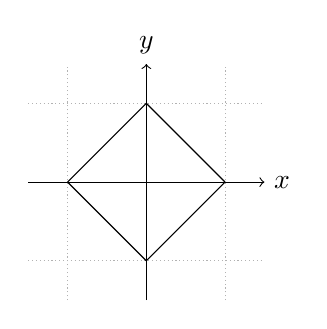
\begin{tikzpicture}
                \draw[style=thin,densely dotted, black!30] (-1.5, -1.5) grid (1.5,1.5);
                \draw[->] (-1.5, 0) -- (1.5,0) node[right] {$x$};
                \draw[->] (0,-1.5) -- (0,1.5) node[above] {$y$};
                \draw (1,0) -- (0,1);
                \draw (0,1) -- (-1,0);
                \draw (-1,0) -- (0,-1);
                \draw (0,-1) -- (1,0);
            \end{tikzpicture}
        \caption{$B_1^1(0,0)$}
        \end{subfigure}

        \begin{subfigure}[c]{.40\textwidth}
            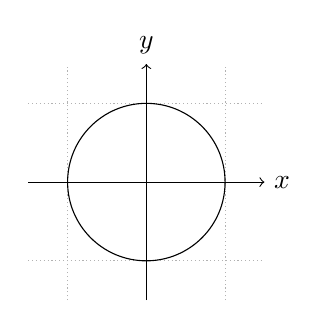
\begin{tikzpicture}
                \draw[style=thin,densely dotted, black!30] (-1.5, -1.5) grid (1.5,1.5);                
                \draw[->] (-1.5, 0) -- (1.5,0) node[right] {$x$};
                \draw[->] (0,-1.5) -- (0,1.5) node[above] {$y$};
                \draw (0,0) circle (1);                
            \end{tikzpicture} 
            \caption{$B_1^2$(0,0)}
        \end{subfigure}
        \begin{subfigure}[c]{.40\textwidth}
            \begin{tikzpicture}
                \draw[style=thin,densely dotted, black!30] (-1.5, -1.5) grid (1.5,1.5);
                \draw[->] (-1.5, 0) -- (1.5,0) node[right] {$x$};
                \draw[->] (0,-1.5) -- (0,1.5) node[above] {$y$};
                \draw (-1,-1) rectangle (1,1);                
            \end{tikzpicture} 
            \caption{$B_1^\infty$(0,0)}
        \end{subfigure}
        \begin{subfigure}[c]{.40\textwidth}
            \begin{tikzpicture}
                \draw[style=thin,densely dotted, black!30] (-1.5, -1.5) grid (1.5,1.5);
                \draw[->] (-1.5, 0) -- (1.5,0) node[right] {$x$};
                \draw[->] (0,-1.5) -- (0,1.5) node[above] {$y$};
                \draw[dashed] (-1,-1) rectangle (1,1);
                \draw[dashed] (1,0) -- (0,1);
                \draw[dashed] (0,1) -- (-1,0);
                \draw[dashed] (-1,0) -- (0,-1);
                \draw[dashed] (0,-1) -- (1,0);п
                \draw (0,0) circle (1);                 
            \end{tikzpicture} 
            \caption{$B_1^p$(0,0)}
        \end{subfigure}
        \caption{Примеры единичных шаров в $l_2^p$}
    \end{figure}
    
    \section{Неполное нормированное пространство}
    \begin{definition}[Финитное линейное пространство]
        \[F = \{ x - \{x_j\}_{j=1}^\infty, x_j \in \bR (\bC) \exists \, N(x) \in \bN : n > N(x) \Rightarrow x_n = 0 \} \]
    \end{definition}
$F \subset l^p \quad 1 \leq p \leq + \infty$.
$(F, || \cdot ||_p) $~--- не полное, $F$~--- не замкнуто.
Будем брать геометрическую прогрессию и обрывать ее на некотором члене.
\begin{gather*}
    x^{(m)} = \left\{ \frac{1}{2}, \frac{1}{4}, \ldots, \frac{1}{2^m}, 0, 0, 0, \ldots \right\} \in F \\
    X = \left\{ \frac{1}{2^k}^\infty_{k=1} \right\} \in l^p \\
    1 \leq p < + \infty \quad ||x - x^{(m)}||_p = \left( \sum^\infty_{k=m+1} \frac{1}{2^{kp}} \right)^{\frac{1}{p}} \underset{m \to \infty}{\longrightarrow} 0
\end{gather*}
Следовательно, $F$~--- не замкнуто.

В качестве упражнения проверить, что $\overline{F}$ в $l^p = ? $ при $p < + \infty$ и при $p = \infty$.
\begin{theorem}
    $C[a,b], ||f||_p = \left( \int^b_a |f(x)|^p dx \right)^{\frac{1}{p}}, 1 \leq p < + \infty$
    \[ (C[a,b], || \cdot || ) \text {~--- не полное } \]
\end{theorem}
\begin{proof}
    При $p = 1$, $[a,b] = [-1,1], f \in C[a,b], \int^b_a |f(x)|^p dx = 0 \Leftrightarrow f(x) \equiv 0$.
    Предъявим фундаментальную последовательность, предел которой не будет непрерывной функцией.

    $f_n = \begin{cases}
        0, -1 \leq x \leq 0 \\
        nx, x \in [0, \frac{1}{n}] \\
        1, x \in [\frac{1}{n}, 1]
    \end{cases}, f \in C[-1,1]$ % тут рисунок f

    $f_n$~--- фундаментальная в $(C[-1,1], p=1)$

    Пусть $ m > n$. %рисунок 2
    \[ \int_{-1}^1 |f_m(x) - f_n(x)| dx = \frac{1}{2} \left( \frac{1}{n} - \frac{1}{m} \right) \leq \frac{1}{2n} \underset{n, m \to \infty}{\longrightarrow} 0 \]

    Пусть $\exists ./ f \in C[-1,1] : \normunder{f-f_n}{1} \underset{n \to \infty}{\longrightarrow} 0$ 
    \begin{gather*}
        m \geq n \quad \int^1_{\frac{1}{n}} \underbrace{|f(x) - 1|}_{=0} dx  \underset{m \to \infty}{\longrightarrow} 0  \\
        \int^1_{\frac{1}{n}} {|f(x) - 1|} dx \leq \int^1_0 |f(x) - f_m(x)|dx \underset{m \to \infty}{\longrightarrow} 0
    \end{gather*}
    $\Rightarrow f(x) = 1, x \in \left[ \frac{1}{n}, 1 \right] \forall n $\\
    \[ \begin{cases}
       \Rightarrow f(x) = 1, x \in (0,1], f \text{ непрерывна }, f(0) = 1\\
        \text{аналогично } f(x) \equiv 0 \text{ на } [-1,0]
    \end{cases} \Rightarrow \text{ противоречие } \]
\end{proof}
\end{document}
